%% LyX 2.3.6.2 created this file.  For more info, see http://www.lyx.org/.
%% Do not edit unless you really know what you are doing.
\documentclass[english,aspectratio=169]{beamer}
\usepackage{mathptmx}
\usepackage{eulervm}
\usepackage[T1]{fontenc}
\usepackage[latin9]{inputenc}
\usepackage{babel}
\usepackage{amstext}
\usepackage{amssymb}
\usepackage{graphicx}
\ifx\hypersetup\undefined
  \AtBeginDocument{%
    \hypersetup{unicode=true,pdfusetitle,
 bookmarks=true,bookmarksnumbered=false,bookmarksopen=false,
 breaklinks=false,pdfborder={0 0 0},pdfborderstyle={},backref=false,colorlinks=true,
 allcolors=NYUPurple,urlcolor=LightPurple}
  }
\else
  \hypersetup{unicode=true,pdfusetitle,
 bookmarks=true,bookmarksnumbered=false,bookmarksopen=false,
 breaklinks=false,pdfborder={0 0 0},pdfborderstyle={},backref=false,colorlinks=true,
 allcolors=NYUPurple,urlcolor=LightPurple}
\fi

\makeatletter


%%%%%%%%%%%%%%%%%%%%%%%%%%%%%% LyX specific LaTeX commands.
%% Because html converters don't know tabularnewline
\providecommand{\tabularnewline}{\\}

%%%%%%%%%%%%%%%%%%%%%%%%%%%%%% Textclass specific LaTeX commands.
% this default might be overridden by plain title style
\newcommand\makebeamertitle{\frame{\maketitle}}%
% (ERT) argument for the TOC
\AtBeginDocument{%
  \let\origtableofcontents=\tableofcontents
  \def\tableofcontents{\@ifnextchar[{\origtableofcontents}{\gobbletableofcontents}}
  \def\gobbletableofcontents#1{\origtableofcontents}
}

%%%%%%%%%%%%%%%%%%%%%%%%%%%%%% User specified LaTeX commands.
\usetheme{CambridgeUS} 
\beamertemplatenavigationsymbolsempty


% Set Color ==============================
\definecolor{NYUPurple}{RGB}{87,6,140}
\definecolor{LightPurple}{RGB}{165,11,255}


\setbeamercolor{title}{fg=NYUPurple}
%\setbeamercolor{frametitle}{fg=NYUPurple}
\setbeamercolor{frametitle}{fg=NYUPurple}

\setbeamercolor{background canvas}{fg=NYUPurple, bg=white}
\setbeamercolor{background}{fg=black, bg=NYUPurple}

\setbeamercolor{palette primary}{fg=black, bg=gray!30!white}
\setbeamercolor{palette secondary}{fg=black, bg=gray!20!white}
\setbeamercolor{palette tertiary}{fg=gray!20!white, bg=NYUPurple}

\setbeamertemplate{headline}{}

\setbeamercolor{parttitle}{fg=NYUPurple}
\setbeamercolor{sectiontitle}{fg=NYUPurple}
\setbeamercolor{sectionname}{fg=NYUPurple}
\setbeamercolor{section page}{fg=NYUPurple}

\AtBeginSection[]{
  \begin{frame}
    \frametitle{Table of Contents}
    \tableofcontents[currentsection]
  \end{frame}

  % \begin{frame}
  % \vfill
  % \centering
  % \begin{beamercolorbox}[sep=8pt,center,shadow=true,rounded=true]{title}
  %   \usebeamerfont{title}\insertsectionhead\par%
  % \end{beamercolorbox}
  % \vfill
  % \end{frame}
}

\makeatother

\begin{document}
\global\long\def\reals{\mathbf{R}}%
 
\global\long\def\integers{\mathbf{Z}}%
 
\global\long\def\naturals{\mathbf{N}}%
 
\global\long\def\rationals{\mathbf{Q}}%
 
\global\long\def\ca{\mathcal{A}}%
 
\global\long\def\cb{\mathcal{B}}%
 
\global\long\def\cc{\mathcal{C}}%
 
\global\long\def\cd{\mathcal{D}}%
 
\global\long\def\ce{\mathcal{E}}%
 
\global\long\def\cf{\mathcal{F}}%
 
\global\long\def\cg{\mathcal{G}}%
 
\global\long\def\ch{\mathcal{H}}%
 
\global\long\def\ci{\mathcal{I}}%
 
\global\long\def\cj{\mathcal{J}}%
 
\global\long\def\ck{\mathcal{K}}%
 
\global\long\def\cl{\mathcal{L}}%
 
\global\long\def\cm{\mathcal{M}}%
 
\global\long\def\cn{\mathcal{N}}%
 
\global\long\def\co{\mathcal{O}}%
 
\global\long\def\cp{\mathcal{P}}%
 
\global\long\def\cq{\mathcal{Q}}%
 
\global\long\def\calr{\mathcal{R}}%
 
\global\long\def\cs{\mathcal{S}}%
 
\global\long\def\ct{\mathcal{T}}%
 
\global\long\def\cu{\mathcal{U}}%
 
\global\long\def\cv{\mathcal{V}}%
 
\global\long\def\cw{\mathcal{W}}%
 
\global\long\def\cx{\mathcal{X}}%
 
\global\long\def\cy{\mathcal{Y}}%
 
\global\long\def\cz{\mathcal{Z}}%
 
\global\long\def\ind#1{1(#1)}%
 %\newcommand{\pr}{P}
\global\long\def\pr{\mathbb{P}}%
 
\global\long\def\predsp{\cy}%
 %{\hat{\cy}}
\global\long\def\outsp{\cy}%

\global\long\def\prxy{P_{\cx\times\cy}}%
 
\global\long\def\prx{P_{\cx}}%
 
\global\long\def\prygivenx{P_{\cy\mid\cx}}%
 %\newcommand{\ex}{E}
\global\long\def\ex{\mathbb{E}}%
 
\global\long\def\var{\textrm{Var}}%
 
\global\long\def\cov{\textrm{Cov}}%
 
\global\long\def\sgn{\textrm{sgn}}%
 
\global\long\def\sign{\textrm{sign}}%
 
\global\long\def\kl{\textrm{KL}}%
 
\global\long\def\law{\mathcal{L}}%
 
\global\long\def\eps{\varepsilon}%
 
\global\long\def\as{\textrm{ a.s.}}%
 
\global\long\def\io{\textrm{ i.o.}}%
 
\global\long\def\ev{\textrm{ ev.}}%
 
\global\long\def\convd{\stackrel{d}{\to}}%
 
\global\long\def\eqd{\stackrel{d}{=}}%
 
\global\long\def\del{\nabla}%
 
\global\long\def\loss{\ell}%
 
\global\long\def\risk{R}%
 
\global\long\def\emprisk{\hat{R}}%
 
\global\long\def\lossfnl{L}%
 
\global\long\def\emplossfnl{\hat{L}}%
 
\global\long\def\empminimizer#1{\hat{#1}^{*}}%
 
\global\long\def\minimizer#1{#1^{*}}%
\global\long\def\optimizer#1{#1^{*}}%
 
\global\long\def\etal{\textrm{et. al.}}%
 
\global\long\def\tr{\operatorname{tr}}%

\global\long\def\trace{\operatorname{trace}}%
 
\global\long\def\diag{\text{diag}}%
 
\global\long\def\rank{\text{rank}}%
 
\global\long\def\linspan{\text{span}}%
 
\global\long\def\spn{\text{span}}%
 
\global\long\def\proj{\text{Proj}}%
 
\global\long\def\argmax{\operatornamewithlimits{arg\, max}}%
 
\global\long\def\argmin{\operatornamewithlimits{arg\, min}}%

\global\long\def\bfx{\mathbf{x}}%
 
\global\long\def\bfy{\mathbf{y}}%
 
\global\long\def\bfl{\mathbf{\lambda}}%
 
\global\long\def\bfm{\mathbf{\mu}}%
 
\global\long\def\calL{\mathcal{L}}%

\global\long\def\vw{\boldsymbol{w}}%
 
\global\long\def\vx{\boldsymbol{x}}%
 
\global\long\def\vxi{\boldsymbol{\xi}}%
 
\global\long\def\valpha{\boldsymbol{\alpha}}%
 
\global\long\def\vbeta{\boldsymbol{\beta}}%
 
\global\long\def\vsigma{\boldsymbol{\sigma}}%
\global\long\def\vtheta{\boldsymbol{\theta}}%
 
\global\long\def\vd{\boldsymbol{d}}%
 
\global\long\def\vs{\boldsymbol{s}}%
 
\global\long\def\vt{\boldsymbol{t}}%
 
\global\long\def\vh{\boldsymbol{h}}%
 
\global\long\def\ve{\boldsymbol{e}}%
 
\global\long\def\vf{\boldsymbol{f}}%
 
\global\long\def\vg{\boldsymbol{g}}%
 
\global\long\def\vz{\boldsymbol{z}}%
 
\global\long\def\vk{\boldsymbol{k}}%
 
\global\long\def\va{\boldsymbol{a}}%
 
\global\long\def\vb{\boldsymbol{b}}%
 
\global\long\def\vv{\boldsymbol{v}}%
 
\global\long\def\vy{\boldsymbol{y}}%

\global\long\def\dom{\textrm{\textbf{dom} }}%
\global\long\def\rank{\text{\textbf{rank }}}%
\global\long\def\conv{\textrm{\textbf{conv} }}%
\global\long\def\relint{\text{\textbf{relint }}}%
\global\long\def\aff{\text{\textbf{aff }}}%

\global\long\def\hil{\ch}%
 
\global\long\def\rkhs{\hil}%
 
\global\long\def\ber{\text{Ber}}%

\global\long\def\softmax{\text{Softmax}}%

\title[DS-GA 1003 ]{Probabilistic models\\
- \\
Bayesian Methods \\
- \\
Discussion}
\author{Marylou Gabri\'e}
\date{March 16, 2021}
\institute{CDS, NYU}

% \title[DS-GA 1003]{Bayesian Methods}
% \author{Julia Kempe \& David S. Rosenberg }
% \date{March 26, 2019}
% \institute{CDS, NYU}

\makebeamertitle
\mode<article>{Just in article version}
\begin{frame}{Bayesian decision for absolute loss is median}
   
 \end{frame}
% 
\begin{frame}{Hours of sun during January in Vienna}
\begin{itemize}
    \item $N=30$ measurements $y_i$
    \item What could you choose as a parametric family?
    \item What is the MLE?
\end{itemize}

\begin{center}
    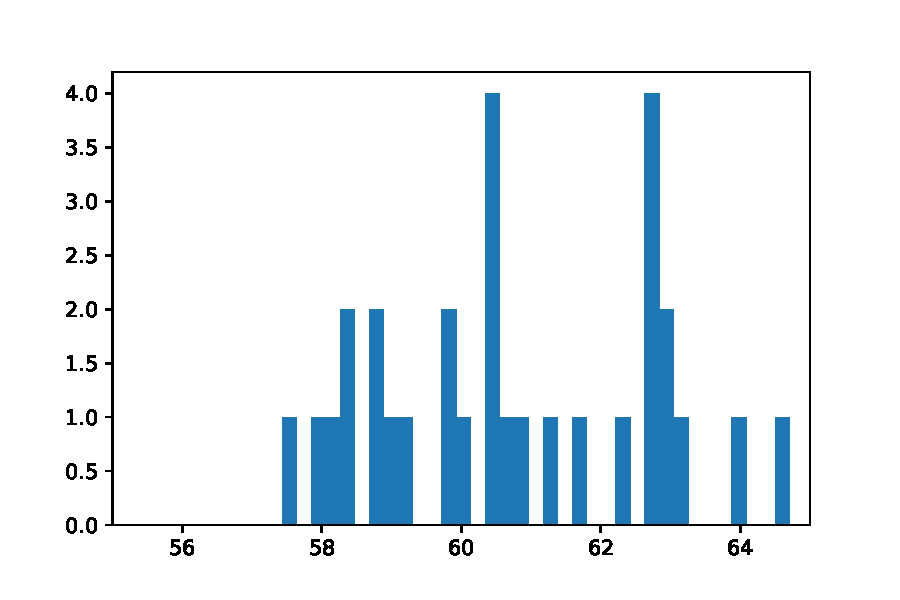
\includegraphics[height=0.75\textheight]{figs/histogram.pdf}
    \par\end{center}
\end{frame}
%
\begin{frame}{Hours of sun during January in Vienna}
    \begin{itemize}
        \item $N=30$ measurements $y_i$
        \item What could you choose as a parametric family?
        \item What is the MLE?
    \end{itemize}
    
    \begin{center}
        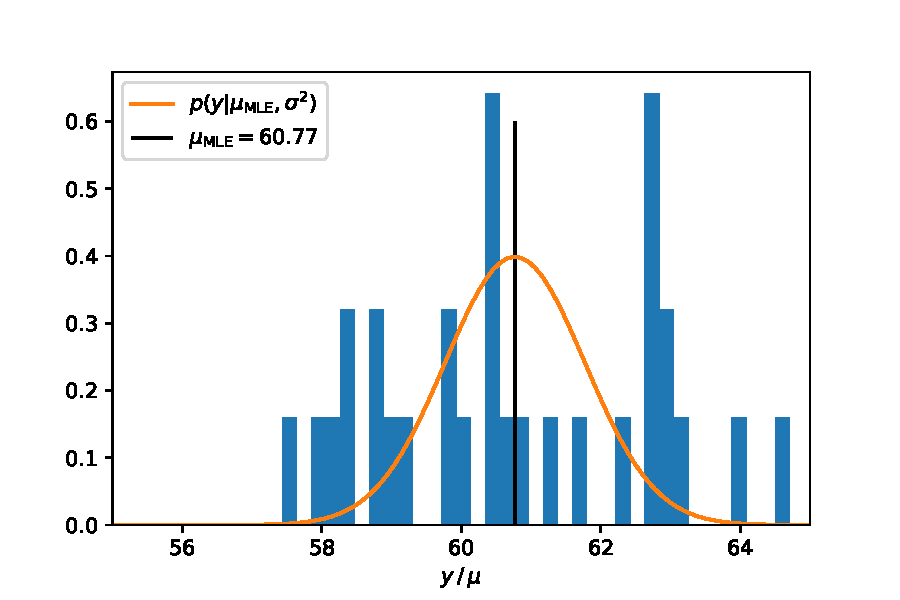
\includegraphics[height=0.75\textheight]{figs/histogram_density.pdf}
        \par\end{center}
\end{frame}
%
\begin{frame}{Hours of sun during January in Vienna}
        \begin{itemize}
            \item $N=30$ measurements $y_i$
            \item Now meteorologists tells you they have a prior: $p(\mu) = \mathcal{N}(\mu; \mu_0,1)$
            \item What is the posterior?
            \item[] 
            \item[] 
            \item[] 
            \item[] 
            \item[] 
            \item[] 
            \item[] 
            \item[] 
            \item[] 
            \item[] 
        \end{itemize}
        
%         \begin{center}
%             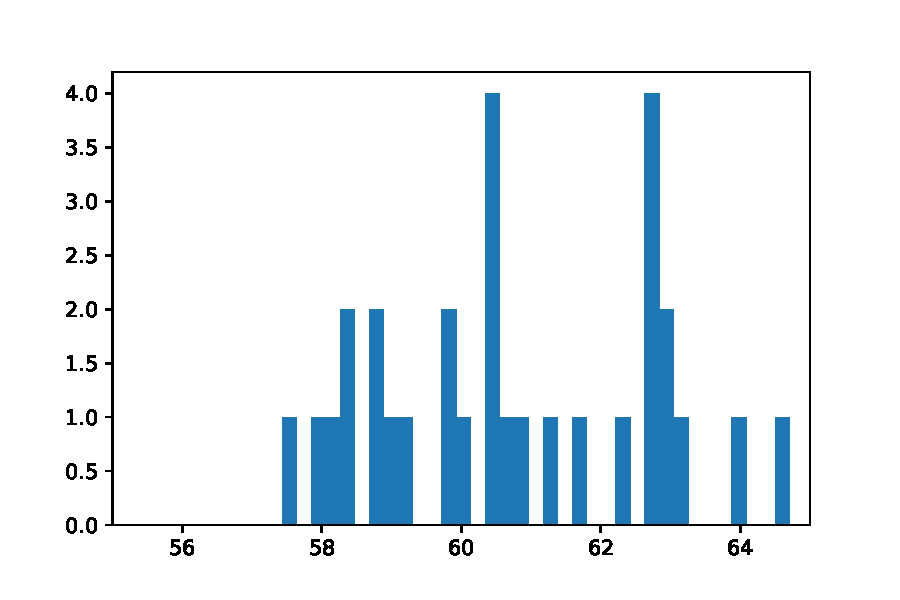
\includegraphics[height=0.75\textheight]{figs/histogram.pdf}
%             \par\end{center}
\end{frame}
%
\begin{frame}{Hours of sun during January in Vienna}
    \begin{itemize}
            \item $N=30$ measurements $y_i$
            \item Now meteorologists tells you they have a prior: $p(\mu) = \mathcal{N}(\mu; \mu_0,1)$
            \item What is the posterior?
    \end{itemize}
    \begin{center}
        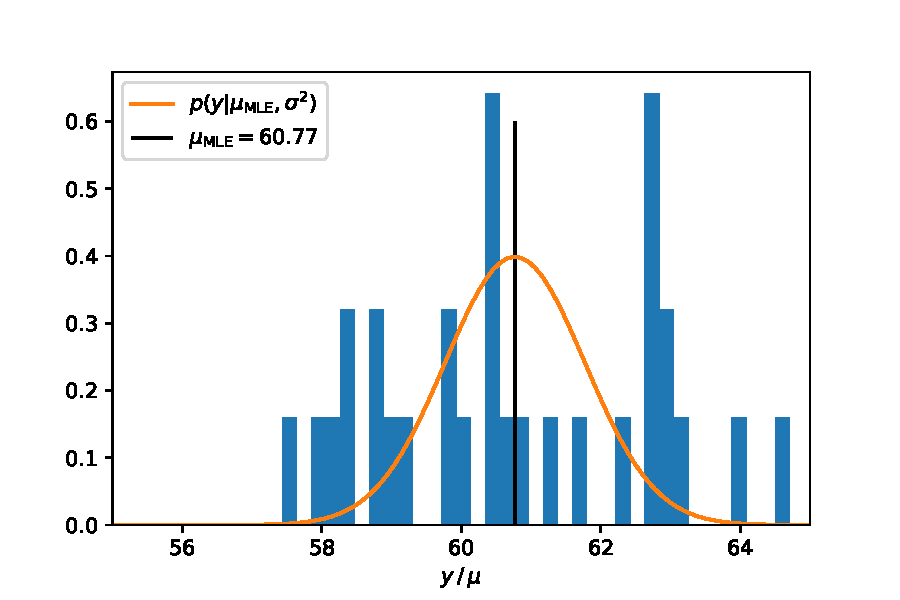
\includegraphics[height=0.55\textheight]{figs/histogram_density.pdf}
        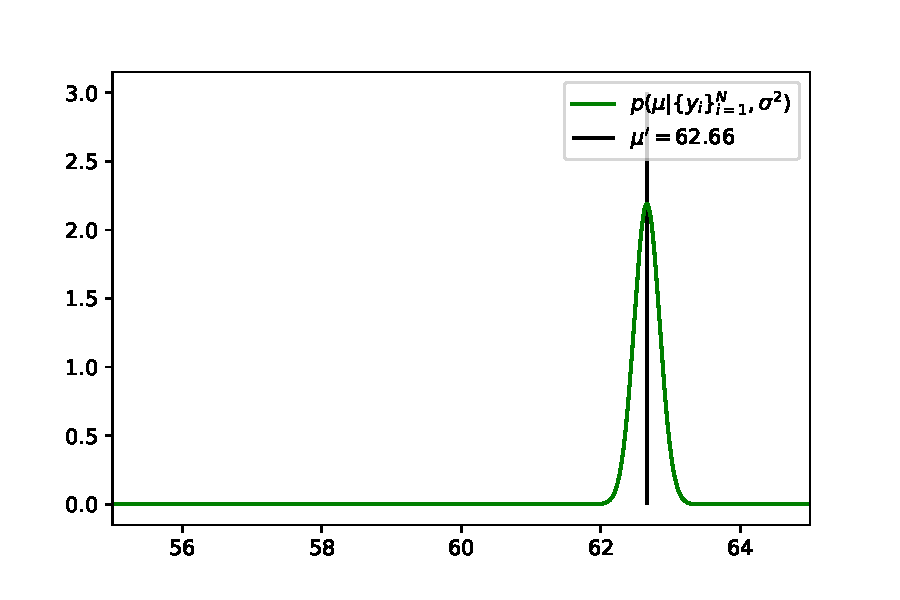
\includegraphics[height=0.55\textheight]{figs/histogram_posterior.pdf}
    \par\end{center}
\end{frame}

\begin{frame}{Hours of sun during January in Vienna}
    \begin{itemize}
            \item $N=30$ measurements $y_i$
            \item Now meteorologists tells you they have a prior: $p(\mu) = \mathcal{N}(\mu; \mu_0,1)$
            \item What is the posterior? What is the credible set?
    \end{itemize}
    \begin{center}
        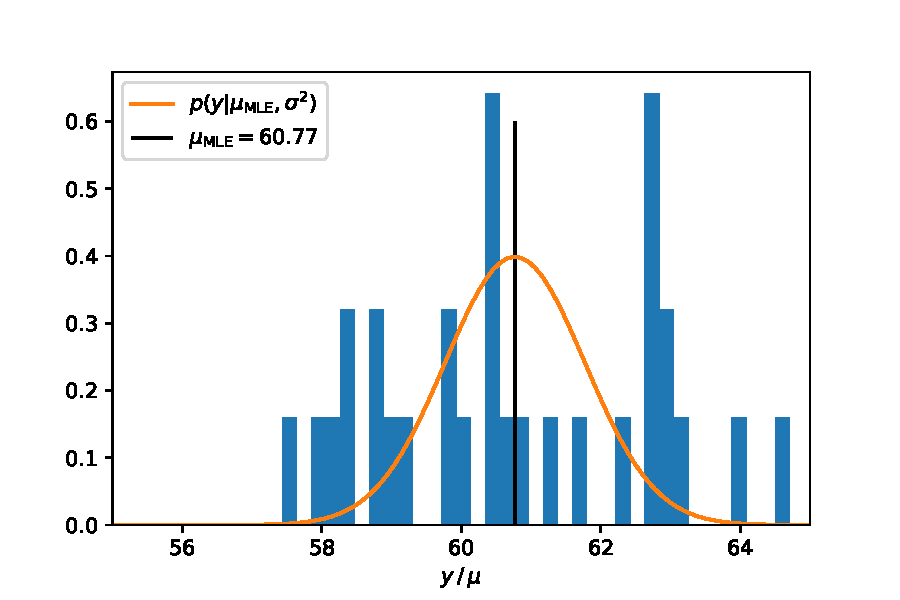
\includegraphics[height=0.55\textheight]{figs/histogram_density.pdf}
        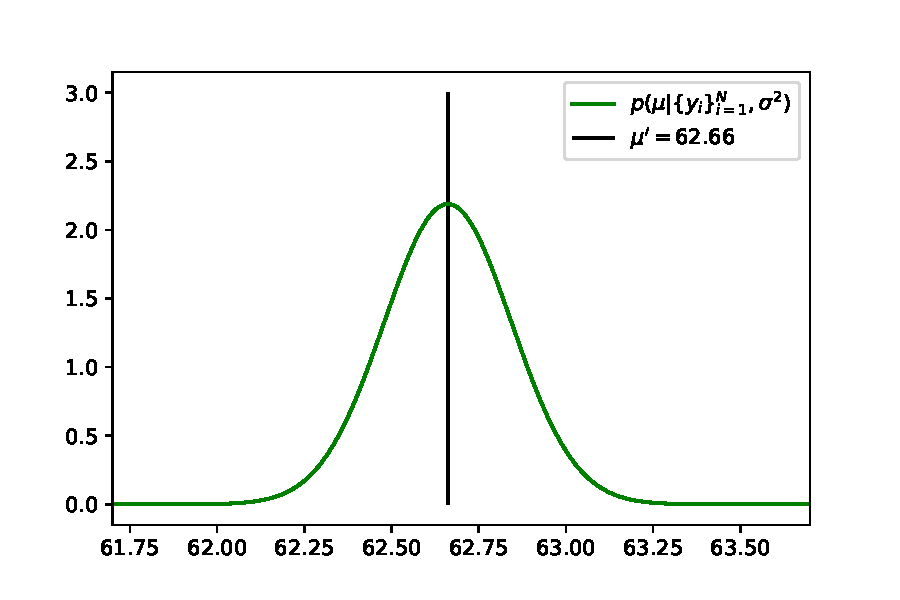
\includegraphics[height=0.55\textheight]{figs/histogram_posterior_zoom.pdf}
    \par\end{center}
\end{frame}

\begin{frame}{Hours of sun during January in Vienna}
    \begin{itemize}
        \item $N=30$ measurements $y_i$
        \item Now meteorologists tells you they have a prior: $p(\mu) = \mathcal{N}(\mu; \mu_0,1)$
        \item The posterior is $p(\mu|\{y_i\}_{i=1}^N, \sigma^2) = \mathcal{N}(\mu; \mu', \sigma'^2)$.
        \item What are the point estimates of $\mu$ minimizing squared loss, absolute loss and 0-1 loss?
        \item[] 
        \item[] 
        \item[] 
        \item[] 
        \item[] 
        \item[] 
        \item[] 
        \item[] 
        \item[] 
    \end{itemize}
\end{frame}

\end{document}

